\section{Introduction}

In recent years, neural networks have had a lot of success in image classification.
This has led to advances in many areas, including computer vision and object recognition.
A.e.advances in a constantly ongoing ImageNet classification challenge, which were achieved
through new approaches,
rather than increasing NNs number of layers and parameters~\cite{russakovsky2015imagenet,DBLP:journals/corr/abs-1905-11946}~.
However, neural networks are also vulnerable to adversarial attacks~\cite{ilyas2019adversarial}.
Adversarial attacks are designed to fool neural networks into misclassifying data.
This can have serious consequences, as it can lead to incorrect results or decisions.
Typical approach to ensure robustness, would be adversarial training, however it can come with a cost of
reduced standard classification accuracy~\cite{https://doi.org/10.48550/arxiv.1805.12152}.
Pretext tasks had shown themselves to be usefully in improving accuracy~\cite{kolesnikov2019revisiting}.
In this research, I would like to evaluate how including state-of-the-art pretext tasks in the training process
influences NNs vulnerability to adversarial attacks.

\subsection{Background}

\paragraph{Adversarial attack}
Goodfellow defined adversarial attacks as “inputs to machine learning models that an
attacker has intentionally designed to cause the model to make a mistake.”
~\cite{DBLP:journals/corr/abs-1802-08195} \\
In the domain of image classification, adversarial attacks are images usually formed by applying a small perturbation
(which is barely noticeable for human viewer) to a naturally occurring image, with intention to make NN miss-classify.
There are many types of adversarial attacks,
and the type of attack depends on the type of model that is being attacked.
In this paper, I focus on the white-box attack, where the attacker has full access to the model and its parameters,
namely Fast Gradient Sign Method.

\paragraph{Fast gradient sign method}
This method was first introduced by Goodfellow and Jonathon Shlens and Christian Szegedy
~\cite{goodfellow2015explaining}.
It produces adversarial images which make NN miss-classify,
but are still recognisable as of the same class for human viewer.
Fast gradient sign method (further denoted as FGSM) works
by using the gradients of the neural network to create an adversarial pattern.
For an input image,
the method evaluates the signed gradient of the loss function with respect to the input image to create a pattern,
which maximises the loss.
The pattern is then added pixel wise to original image.
The new image is called the adversarial image.
The process can be summarised using the following expression:
\begin{equation}
    adv\_x = x + \epsilon \cdot sign(\nabla_x J(\theta, x, y))
\end{equation}
(where $\epsilon$ denotes the intensity of adversarial pattern).
\\
\begin{figure}[h]
    \begin{subfigure}{0.4\textwidth}
        \caption{Tulips 40\% confidence}
        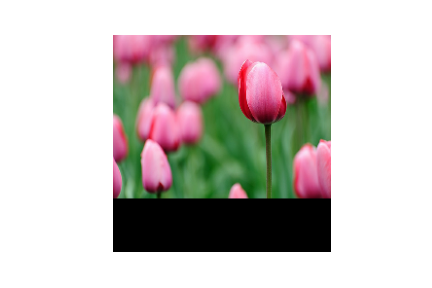
\includegraphics[width=8cm]{images/og_image}
    \end{subfigure}
    \begin{subfigure}{0.4\textwidth}
        \caption{Adversarial pattern for this image}
        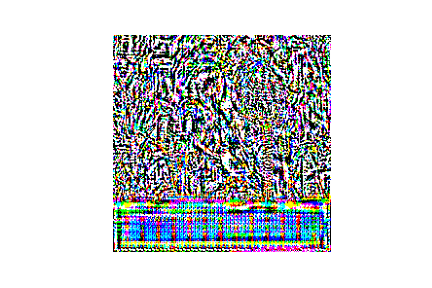
\includegraphics[width=8cm]{images/adv_pattern}
    \end{subfigure}
    \\
    \begin{subfigure}{0.4\textwidth}
        \caption{$\epsilon = 0.01$, Roses 40\% confidence}
        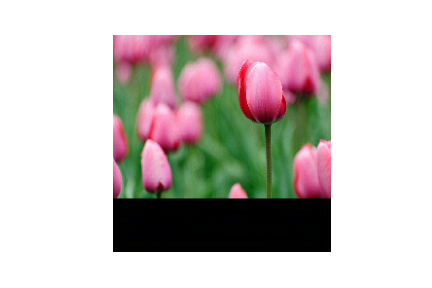
\includegraphics[width=8cm]{images/adv_attack_001}
    \end{subfigure}
    \begin{subfigure}{0.4\textwidth}
        \caption{$\epsilon = 0.1$, Roses 40\% confidence}
        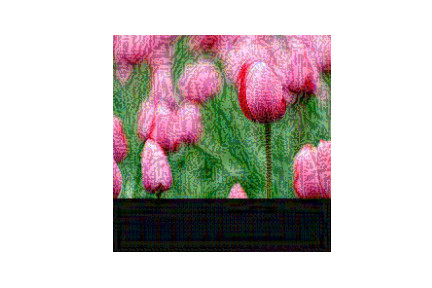
\includegraphics[width=8cm]{images/adv_attack_01}
    \end{subfigure}
\end{figure}

\paragraph{Pretext task}
Pretext task is the self-supervised learning task solved to learn visual representations,
with the aim of using the learned representations or model weights obtained in the process, for the downstream task.
It has been showm, that pretext tasks can significantly improve NNs accuracy.~\cite{kolesnikov2019revisiting}
It is also believed they contribute to NNs learning of important (as per human agents) features.
In this paper I focus on rotation and jigsaw pre-text tasks.

\paragraph{Rotation pretext task}
A common choice of pretext task could be to produce 4 copies of
a single image by rotating it by {0°, 90°, 180°, 270°} and let a single network predict the rotation which was applied.
Alexander Kolesnikov and Xiaohua Zhai and Lucas Beyer: "Intuitively, a good model should learn to
recognize canonical orientations of objects in natural images" ~\cite{kolesnikov2019revisiting}.

\paragraph{Jigsaw pretext task}
The task is
to recover relative spatial position of 4 sampled image patches
after a random permutation of these patches was performed
~\cite{kolesnikov2019revisiting}.
All of these patches are concatenated in 'puzzle' image,
which is later sent through same network, which needs to predict a permutation applied.



\section{Methods}

\paragraph{Model}
Convolutional networks' architectures for image recognition have evolved quite drastically in recent years,
with numerous options available "out of the box".
A.e.\ Efficient Net (further denoted as EffNet) delivers impressive accuracy,
while being able to scale better than a lot of previous architectures~\cite{DBLP:journals/corr/abs-1905-11946}.
For this paper, the evaluation was done using it, namely EfficientNetB0
\footnote{For details about EfficientNet usage please refer to \href{https://keras.io/api/applications/efficientnet/}{keras/efficientnet}}.

\paragraph{Rotation pretext task}
Each image from original dataset was rotated 0°, 90°, 180°, 270° and assigned new pseudo label from [0, 1, 2, 3] accordingly.
All 4 batches of rotated images, as well as pseudo labels were concatenated in new dataset, and shuffled.
Then the last dense layer of NN was replaced with a dense layer for the corresponding number of pseudo classes (4).
Then the same model was then trained to identify rotation applied.
\begin{figure}[h]
    \begin{subfigure}{0.33\textwidth}
        \caption{Label = 0}
        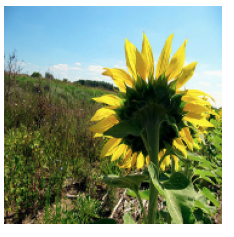
\includegraphics[width=5cm]{images/rot_0}
    \end{subfigure}
    \begin{subfigure}{0.2\textwidth}
        \caption{Label = 1}
        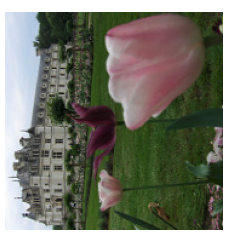
\includegraphics[width=5cm]{images/rot_1}
    \end{subfigure}
    \begin{subfigure}{0.33\textwidth}
        \caption{Label = 2}
        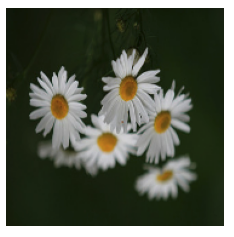
\includegraphics[width=5cm]{images/rot_2}
    \end{subfigure}
    \caption{An example how images used for rotation pretext task could look like}
\end{figure}




\paragraph{Jigsaw pretext task}For jigsaw,
a similar approach as described by Mehdi Noroozi and Paolo Favaro~\cite{DBLP:journals/corr/NorooziF16} was adopted.
Random 4 out of 24 possible permutations were chosen for each batch (number of possible permutation can be obtained from Newtonian binomial $P=\frac{r!}{(r-n)!}$).
For each permutation, each image was cut in 4 equal parts,
afterwards these tiles were permuted according to chosen permutation, and concatenated in 1 (puzzle) image.
Similarly, to rotation pseudo labels in [0\ldots23] had been assigned,
images were shuffled, and the last dense layer was replaced by a suitable one.
The network then is trained to identify permutation applied \footnote{
    For detailed implementation of pretext tasks as well as adversarial attack \\ using FGSM please refer to \href{https://github.com/Goofy-Goof/ISS/blob/33a2ad40b779ff230aae31c29d2edc2cf5d90406/impl}{GitHub/impl}.
}.
\\
\begin{figure}[h]
    \begin{subfigure}{0.33\textwidth}
        \caption{Original image}
        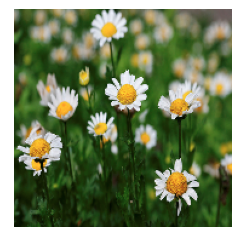
\includegraphics[width=5cm]{images/dandelion}
    \end{subfigure}
    \begin{subfigure}{0.2\textwidth}
        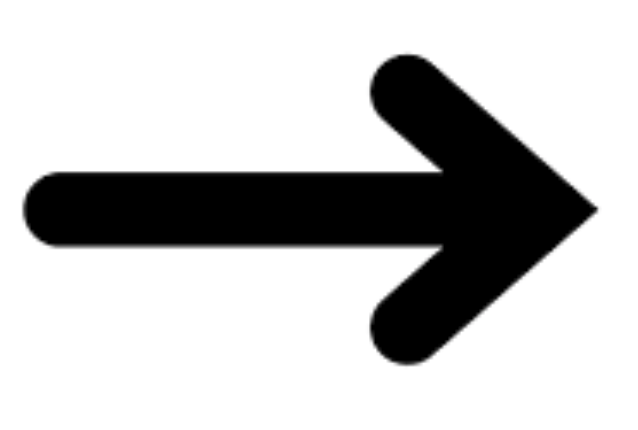
\includegraphics[width=3cm]{images/arrow}
    \end{subfigure}
    \begin{subfigure}{0.33\textwidth}
        \caption{Generated puzzle, label=1}
        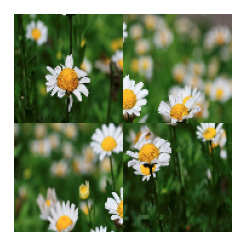
\includegraphics[width=5cm]{images/puzzle}
    \end{subfigure}
    \caption{An example how puzzle for jigsaw pretext task could look like}
\end{figure}

\paragraph{Transfer learning}
For transfer learning EffNet was pre-trained on "imagenette" dataset for image classification.
Imagenete is a selection of 10 classes from the widely known ImageNet dataset. \footnote{
    For information about "imagenette" please refer to \href{https://www.tensorflow.org/datasets/catalog/imagenette}{TF/imagenette}
}

\paragraph{Adversarial Images with FGSM}
My implementation of FGSM was based on \href{https://www.tensorflow.org/tutorials/generative/adversarial_fgsm}{TF FGSM}.
In order to generate adversarial pattern for each image,
gradient of loss function is evaluated with sign for each image.
Then according to this formula:
\begin{equation}
    adv\_x = x + \epsilon \cdot sign(\nabla_x J(\theta, x, y))
\end{equation}
pattern was then added pixel wise to original image with $\epsilon = 0.01$.
Resulting adversarial image was then clipped by value, so each pixel value stays in interval [0\ldots255],
as required for RGB color encoding.

\paragraph{Evaluation approach}
In order to evaluate, how including pretext task in the training process influences NNs vulnerability against adversarial attacks,
I have measured miss-classification rate while keeping the intensity of adversarial pattern fixed at $\epsilon = 0.01$.
\\
Following metrics of interest were recorded:

\begin{equation}
    Accuracy_i = \frac{\# \; images \; correctly \; classified_i}{\# \; test \; images_i} \cdot 100 \%
\end{equation}
\begin{equation}
    \overline{Accuracy} = \frac{1}{N}  \sum_{i=1}^{N}{Accuracy_i}
\end{equation}
\begin{equation}
    Miss \; rate_i = \frac{\# images \; miss \; classified_i}{\# \; images \; correctly \; classified_i} \cdot 100 \%
\end{equation}
\begin{equation}
    \overline{Miss \; rate} = \frac{1}{N}  \sum_{i=1}^{N}{Miss \; rate_i}
\end{equation}
\\
The dataset "tf\_flowers" was chosen for experiment, 5\% of dataset were reserved for evaluation.
\footnote{For information about "tf\_flowers" please refer to \href{https://www.tensorflow.org/datasets/catalog/tf_flowers}{TF/tf\_flowers}}
\\
During each evaluation round NN network was pre-trained either with transfer learning, or rotation, or jigsaw.
The number of training epochs was varied in [15, 30, 45, 60] for pretext training, while the number of epochs for downstream
training was fixed at 30.
\\
Reserved images were given to NN, the correctly classified ones were saved for later use.
Then, for each saved (previously correctly classified) image adversarial example was generated
using FGSM with $\epsilon = 0.01$.
\\
The number of correct classifications, as well as the number of miss-classifications were recorded at the end of each round.
